\documentclass{article}
\usepackage{lmodern}
\usepackage[T1]{fontenc}
\usepackage{upquote}
\usepackage{amsmath}
\usepackage{amssymb}
\usepackage{wasysym}
\usepackage{color}
\usepackage{epsfig}
\usepackage{arydshln}
\usepackage{hyperref}
\setlength{\oddsidemargin}{0in}\setlength{\textwidth}{6.5in}
\setlength{\topmargin}{0.0in}\setlength{\textheight}{8.5in}
\input{cs418-macros}
\newcommand{\srcdir}{https://www.students.cs.ubc.ca/~cs-418/2025-1/hw/5/src}
\newcommand{\sq}{\textquotesingle}
\newcommand{\bsq}[1]{\textquotesingle#1\textquotesingle}
%\newcommand{\erlist}[1]{[#1]}
%\newcommand{\erldoc}[3]{\hrefc{http://erlang.org/doc/man/#1.html\##2-#3}{#2}}
%\newcommand{\erlangdoc}[2]{\hrefc{http://erlang.org/doc/man/erlang.html\##1-#2}{#1}}
%\newcommand{\listdoc}[2]{\hrefc{http://erlang.org/doc/man/lists.html\##1-#2}{lists:#1}}
%\newcommand{\iodoc}[2]{\hrefc{http://erlang.org/doc/man/io.html\##1-#2}{lists:#1}}
%\newcommand{\addpath}{\hrefc{http://erlang.org/doc/man/code.html\#add_path-1}{code:add\_path}}
\newcommand{\erltemplate}{\hrefc{http://www.students.cs.ubc.ca/~cs-418/2025-1/hw/5/src/hw5.erl}{\code{hw5.erl}}}
\newcommand{\erlprompt}{>~}
\newcommand{\SpeedUp}{\ensuremath{\mathit{SpeedUp}}}
\newcommand{\ro}{{\color{MediumRed}{1}}}
\newcommand{\bz}{{\color{blue}{0}}}
\newcommand{\Henon}{H\'{e}non}
\newcommand{\gpumodel}{RTX 3070 Ti}

\newenvironment{answer}
{\par\color{blue}}
{\normalfont\par}

\newcounter{saveenumii}
\begin{document}
\noindent%
CpSc 418 \hfill \begin{tabular}[t]{c}{\Large\bf Homework 5}\smallskip \\
\end{tabular}
\hfill Due: Nov. 14, 2025, 11:59pm\\
\hfill Early Bird: Nov. 12, 2025, 11:59pm\medskip\\
\textbf{142 points +1 extra credit)}\medskip\\
Please submit your solution using handin:\\
\rule{2em}{0ex}\texttt{handin cs-418 hw5}\\
Your solution should have three files file: \texttt{hw5.pdf}.

\section*{The Questions}

\begin{enumerate}\setcounter{enumi}{-1}
    \item \textbf{Collaborators} (\textbf{2 points (+1 extra credit)}).\label{q:collab}\\
          In your \texttt{hw4.pdf} list anyone you collaborated with or outside materials that you used.
          \begin{itemize}
              \item If the collaborator is a student in this class, give their CWL.
              \item If the colloborator is a human who is not in this class, give their name
                    and a short (i.e.\ one sentence) description of their relevance to this course.
              \item If you used on-line material, give the URL.
              \item If you used an AI assistant, give the name of the assistant.
                    We'll give extra credit if you include your prompt, and one sentence to say
                    what was useful in the response.
              \item Other sources such as books should be just cited clearly.
          \end{itemize}
          For each collaborator, list what questions you collaborated on.
          \par
          You do not need to list course materials including anything on the
          \hrefc{https://www.students.cs.ubc.ca/~cs-418}{cs-418 website},
          assigned readings, the official \hrefc{https://www.erlang.org}{Erlang} documentation,
          or material from office hours or tutorials.
          \par
          If you had no collaborators, write ``\textit{No collaborators}''.
          A blank or omitted response will get no credit.
          \par
          \textbf{Extra Credit:} When grading HW 1, one of our TA's pointed out that many of
          you did an extra fantastic job on this question providing detailed prompts that
          you used with AI assistants.  We really appreciate this as we are learning how
          we can best leverage emerging technologies in our teaching.  In fact, we appreciated
          it so much that we gave a point of extra credit for answers that the TA flagged
          as extra good!  Thanks.

          Going forward, we want to make this opportunity to everyone, whether or not you use AI.
          Here are \emph{five} ways you can get that extra credit point:
          \begin{enumerate}
              \item Include your prompts to AI assistants as described above.
              \item Tell us why you didn't use an AI assistant or didn't find it helpful.
              \item Write a few sentences that you think would be the best advice you could
                    give to a student starting this assignment based on your experience of
                    completing it.
              \item Identify a question that you thought was particularly helpful or
                    pointlessly tedious, and give us a few sentences saying why.
              \item Write something else that you think is worthy of extra-credit.
                    Mark it clearly as your response to the \textbf{Extra Credit} part
                    of this question.
          \end{enumerate}
    \item Branch Prediction: (\textbf{35 points})\label{q:branch}\\
          Superscalar processors can execute multiple instructions in a single clock cycles.
          Typical programs have branches every 5 to 10 instructions, and processors tend to have
          deep execution pipelines; it can take five to ten or more clock cycles from fetching an
          instruction until its result is available.
          Conditional and computed branches are a headache for computer architects because we don't
          know what instruction to fetch next until the branch instruction completes.
          For example, if a branch takes five clock cycles to complete, and the superscalar processor
          fetches four instructions per clock cycles, \emph{twenty} instructions will be fetched between
          fetching a branch and knowing its outcome.  This likely included a few more branches!
          \par
          To address these issues, superscalar processors use branch prediction.
          A simple predictor simply counts the number of times the branch is taken or not.
          The counter is incremented if the branch is taken, and decremented when it is not taken.
          For example, we could have a three bit counter that saturates at \code{+3} or \code{-4}.
          If a branch is taken, and the counter is already at \code{+3}, it stays at \code{+3}.
          Likewise for decrementing the counter when the branch is not taken.
          When the branch is fetched, if the branch is predicted to be taken,
          the processor jumps to fetching from the branch target, and if the branch is predicted as untaken,
          the processor continues fetching the instructions immediately after the branch.
          See the reading on superscalar processors or the
          \hrefc{https://wwww.students.cs.ubc.ca:~cs-418/2025-1/lecture/10-06/slides.pdf}{Oct.\ 6} slides
          for more details.
          \par
          This problem explores the cost of branch misprediction.
          The key function for this is \code{ar\_op} in \hrefc{\srcdir/array.c}{\texttt{array.c}}.
          If we look at the assembly code for the \code{ar\_op} function,
          we find a conditional branch corresponding to the \code{i <  n-7}
          test of the \code{for}-loop, and a computed branch corresponding
          to the \code{switch} statement.

          \begin{enumerate}
              \item (\textbf{10 points})
                    Assume that the branch corresponding to \code{i < n-7} is \emph{taken} when
                    \code{i < n-7} and not taken when \code{i >= n-7}.
                    This is a slight simplification; in the actual assembly code, there is one branch at
                    the beginning of the \code{ar\_op} function to make sure \code{n-7 >= 0}, and then
                    a branch at the end of the for-loop body to branch back to the start of the loop body
                    if \code{i < n-y}.
                    \par
                    With the assumptions of described in the previous paragraph, consider a call to
                    \code{ar\_op(op, n)} \code{n > 7}.
                    \begin{enumerate}
                        \item (\textbf{2 points}) How many times in total is the branch taken for this call to \code{ar\_op}?
                              \begin{answer}
                                  n-7 times.
                              \end{answer}
                        \item (\textbf{2 points}) How many times in total is the branch not-taken for this call to \code{ar\_op}?
                              \begin{answer}
                                  1 time.
                              \end{answer}
                        \item (\textbf{6 points}) If the branch-predictor uses the saturating counter method described above,
                              what fraction of the \code{i < n-7} branches will be predicted correctly?\\
                              Provide a brief (one or two sentences) justification for your answer.
                              \begin{answer}
                                  \begin{displaymath}
                                      \left\{
                                      \begin{array}{ll}
                                          \frac{0}{1}      & \text{if } n \leq 7 \\[5pt]
                                          \frac{n-7}{n-6}, & \text{otherwise }
                                      \end{array}
                                      \right.
                                  \end{displaymath}
                                  Since the incrementor starts at 0 and increases to 3, it will only be incorrect one time and that is when $i = n - 7$. So it will correctly predict $n - 7$ out of $n - 6$ branches.
                              \end{answer}
                    \end{enumerate}

              \item (\textbf{5 points})
                    Consider the branch corresponding to the switch statement, i.e.\ the branch
                    that can go to one of eight \code{case}s depending on the value of
                    \code{op[i + (acc \& y)]}.  For simplicity, assume that the branch predictor
                    guesses that the branch goes to same place as the previous time the branch was executed.
                    \begin{enumerate}
                        \item (\textbf{2 points}) If all elements of \code{op} are the same,
                              for example \code{op[i] = 0} for all \code{0 <= i < n}, what fraction of the
                              \code{op[i + (acc \& y)]} branches will be predicted correctly?
                        \item (\textbf{3 points}) If the elements of \code{op} are uniformly random with
                              \code{0 <= op[i] < 8} for all \code{0 <= i < n}, what fraction of the
                              \code{op[i + (acc \& y)]} branches will be predicted correctly?
                              \par
                              Note: this is only an approximation because there is some correlation of
                              \code{acc \& 7} and \code{prev \& 7}.  We will ignore that.
                    \end{enumerate}

              \item (\textbf{15 points})
                    Compile and run \texttt{op}  on \code{thetis.students.cs.ubc.ca} or
                    \code{gambier.student.cs.ubc.ca}.  The command\\
                    \rule{1.5em}{0ex}\texttt{./op 1000 100 10000 const0}\\
                    will give the mean and standard deviation for the time to execute \code{ar\_rand}
                    with \code{n=1000} and randomly distributed elements for \code{op}.
                    In a bit more detail, the command is\\
                    \rule{1.5em}{0ex}\texttt{./op n\_op ntrials runs\_per\_trial dist}\\
                    where
                    \begin{description}
                        \item{\code{n\_op}}: number of elements in the \code{op} array.
                        \item{\code{n\_trials}}: Perform \code{ntrials} timing measurements.
                              Report the mean and standard deviation.
                        \item{\code{runs\_per\_trial}}: Each timing measurement consists of
                              calling \code{ar\_op(op, n\_op)} \code{runs\_per\_trial} times.
                              The total time for each measurement is dividdd by \code{runs\_per\_trial}
                              to get a value for the time per call to \code{ar\_op}.
                              This is because the time for an individual call is short enough to introduce
                              large clock quantization errors.
                        \item{\code{dist}}: The distribution to use for the elements of \code{op}.
                              \code{dist="rand"} generates random elements with each element in \code{0}, \ldots, \code{7}.
                              \code{dist="constN"} where \code{N} is a decimal digit sets each element to \code{N}.
                              \code{"c"} is an abbreviation for \code{"const0"}.
                    \end{description}
                    \begin{enumerate}
                        \item (\textbf{5 points}) Include a table of your raw timing data for your answers to this the remaining
                              parts of this question.
                        \item (\textbf{5 points}) By running \texttt{./op} with random and constant distributions for the elements
                              of \code{op}, determine the branch mispredict penalty, in nanoseconds,
                              for executions on \code{gambier} or \code{thetis}.
                        \item (\textbf{5 points}) The Intel Xeon E5-2698 v3 processors in \texttt{thetis} and \texttt{gambier}
                              have a base CPU clock frequency of 2.3GHz and a boost-clock frequency of 3.6GHz.
                              How many clock-cycles is the branch-mispredict penalty if the CPU is operating at the base clock?
                              How many clock-cycles is the branch-mispredict penalty if the CPU is operating at the boost clock?
                              \par
                              If \texttt{thetis} or \texttt{gambier} is lightly loaded, you should see the boost-clock
                              performance, but I'm not absolutely certain of that.
                    \end{enumerate}

              \item (\textbf{5 points})
                    I count 14 to 18 x86 instructions per iteration of the \code{for(i=0; \ldots)} loop in
                    \code{ar\_op}.  Let's take the midpoint of 16 instructions per iteration.
                    Assuming the boost clock rate of 3.6GHz, how many instructions does the \texttt{thetis}
                    or \texttt{gambier} execute per clock cycle based on your data above?
                    \par
                    Note: the number that you get from this estimate is probably a bit high.
                    The x86 internally translates x86 instructions into ``simpler'', ROPs, roughly RISC instructions.
                    In the process, it appears to do some local optimizations.
                    For example, I expect that it figures out how eliminate some of the inefficiencies that occur
                    because the x86 instruct set only has eight programmer visible registers.
                    The ROP count might be closer to 9 to 12 operations per loop iteration,
                    but I don't know of a way to check the details.
          \end{enumerate}


          \begin{figure}\begin{center}
                  \begin{xcode}xxxx\=xxxx\=xxxx\=xxxx\=xxxx\=\kill
                      int ar\_op(int *op, int n) \{\+\\
                      int prev = 0, acc = 0, next = 0;\\
                      for(int i = 0; i < n-7; i++) \{\+\\
                      switch (op[i + (acc \& 7)]) \{\+\\
                      case 0: next = prev + acc; break;\\
                      case 1: next = prev - acc; break;\\
                      case 2: next = prev \& acc; break;\\
                      case 3: next = prev | acc; break;\\
                      case 4: next = prev \textasciicircum{} acc; break;\\
                      case 5: next = acc + 0x1357; break;\\
                      case 6: next = acc \textasciicircum{} 0x1357; break;\\
                      case 7: next = acc <{}< 11; break;\\
                      \}\-\\
                      prev = acc;\\
                      acc = next;\\
                      \}\-\\
                      return(acc);\\
                      \}\-\\
                  \end{xcode}
                  \caption{The \code{ar\_op} function for Question~\ref{q:branch}}
              \end{center}\end{figure}

    \item Dynamic Programming (\textbf{37 points})\label{q:dp}
          For \hrefc{https://www.students.cs.ubc.ca/~cs-418/2025-1/hw/4/hw4.pdf}{Homework 4},
          you examined the performance of dynamic programming using the work-span model.
          The work-span approach gives shows the dependencies in dynamic programming which
          indicates how one \emph{could} make a parallel implementation.
          The work-span model ignores communication cost.
          To obtain an \emph{efficient} implementation, we need to find a way to assign
          tasks to processors and account for the communication costs.

          One approach to implementing a parallel version of dynamic programming
          is to partition the tableau into ``tiles''.
          If each tile has $N_{tr}$ rows and $N_{tc}$ columns,
          then a process will perform $N_{tr}N_{tc}$ work before needing
          to communicate with adjacent tiles.  This allows us to amortize the communication costs.

          \begin{enumerate}
              \item Implement a parallel version of dynamic programming for the editing-distance problem
                    (\textbf{15 points}).\\
                    The file \hrefc{https://www.students.cs.ubc.ca/~cs-418/2025-1/hw/5/src/hw5.erl}{hw5.erl}
                    provides template code, and
                    \hrefc{https://www.students.cs.ubc.ca/~cs-418/2025-1/hw/5/src/hw5_lib.erl}{hw5\_lib.erl}
                    provides:
                    \begin{itemize}
                        \item A sequential implementation of dynamic programming for your reference.
                              This is also useful for tests.  Some of you may find it to be a useful example
                              if you need to review dynamic programming.
                        \item Functions for handling a single ``tile'' of the dynamic programming tableau.
                              That's right -- we've given you most of the sequential code that you need, you
                              just need to make it parallel.
                        \item Functions for working with chains of processes.
                              That's right -- we're even giving you the low-level parallel code.
                              My implementation uses such a chain.
                        \item Why chains of processes?  Think about the work-span model for the parallelism
                              available in dynamic programming that you worked out in Homework 5.
                              There is an ``obvious'' way to write a parallel version that uses one process for
                              each tile, but this is very inefficient because most of the processes are idle most of the time.
                              What is the maximum number of processes that can be active at one time?
                              Call this $P_{\max}$.
                              Can you implement your parallel version using $P_{\max}$ processes?
                    \end{itemize}
                    The \code{hw5:ed\_par} function takes a parameter of \code{TileWidth}.
                    That might be specific to my implementation.  If you need different
                    parameters for configuring your implementation, please make a private post
                    to piazza.  We'll work it out.
              \item Write a one to three paragraph describing your parallel implementation
                    (\textbf{5 points}).\\
                    This should be sufficient to make it easy for another programmer to understand your solution.
                    You can see the comments in
                    \hrefc{https://www.students.cs.ubc.ca/~cs-418/2025-1/hw/1/src/hw5_lib.erl}{hw5\_lib.erl}
                    as an example.
                    In fact, more than half of the lines in
                    \hrefc{https://www.students.cs.ubc.ca/~cs-418/2025-1/hw/5/src/hw5_lib.erl}{hw5\_lib.erl}
                    are comments.
                    You may not need to be that thorough, but you should make your design choices clear.
              \item Write some test-cases for \code{hw5:ed\_par}. (\textbf{5 points})\\
                    Feel free to use \code{hw5\_lib:ed\_seq} as a reference.
                    If you used \code{hw5\_lib:default\_op\_costs()}, round-off error shouldn't affect your
                    results, and that will make comparisons easier.\\
                    If you wrote other functions, provide tests for them as well.
              \item Measure and report speed-up. (\textbf{12 points})\\
                    As usual, please run your timing measurements on
                    \texttt{gambier.students.cs.ubc.ca} or\\
                    \texttt{thetis.students.cs.ubc.ca}.
                    Use test cases where the time for \code{hw5\_lib:ed\_seq} is up to one second.
                    I found that I could have strings of 1000 to 2000 characters and satisfy this constraint.
                    \begin{enumerate}
                        \item Include your raw data. (\textbf{4 points})
                        \item Show how your choices of configuration parameters impact the result. (\textbf{3 points})\\
                              For my solution, there is some impact on changing the number of processes or the tile width,
                              but the region of optimal performance is pretty flat.
                        \item Report the best speed-up you could get (\textbf{2 points})\\
                              Note: I got a speed-up of about 8 on \code{thetis} with 32, 2-way multithreaded cores.
                              Running on my laptop (M1-Pro CPU, 8 cores), I get a speed-up of about 5.
                        \item Identify causes of performance loss for this example? (\textbf{3 points})\\
                              You may need to speculate, but give some evidence for your guesses.
                    \end{enumerate}
          \end{enumerate}


          \begin{figure}\begin{center}
                  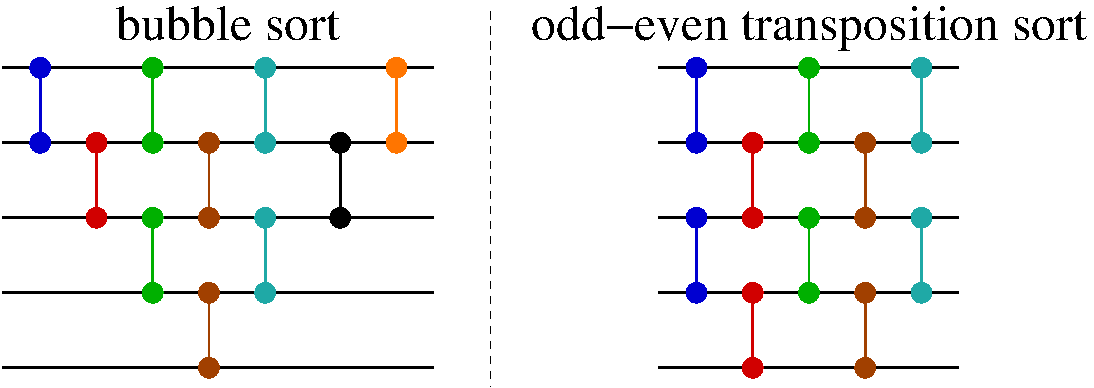
\includegraphics[height=3cm]{figs/sort.pdf}
                  \caption{Sorting networks for a linear array}\label{fig:sort}
              \end{center}\end{figure}.

    \item Sorting on a linear array. (\textbf{20 points})\label{q:sort-linear}\\
          \newcommand{\xj}[1]{\ensuremath{x_{#1}}}
          \newcommand{\xji}[2]{\ensuremath{\xj{#1}[#2]}}
          \newcommand{\cth}[1]{\ensuremath{\code{#1}^{th}}}
          Figure~\ref{fig:sort} shows two sorting networks for sorting and array of five elements.
          These can be implemented on a linear-array of processors, and each compare-and-swap element
          only compares two adjacent elements in the network.
          Of course, they can be implmented on higher-dimensional networks such as meshes, hypercubes, or the Dragonfly;
          they don't \emph{need} all of the connectivity that those fancier networks provide.
          The bubble-sort and odd-even transposition sorting networks can be generalize for an arbitrary number of
          inputs, $N$ as seen in the \code{hw5:bubble/1} and \code{hw5:odd\_even/1};
          see \erltemplate{}.
          \begin{enumerate}
              \item (\textbf{4 points}): What are the work and span for the bubble-sort and
                    odd-even transposition sort networks with five inputs as shown in Figure~\ref{fig:sort}:
                    \begin{enumerate}
                        \item (\textbf{1 point}) Work for \code{bubble(5)}:
                        \item (\textbf{1 point}) Span for \code{bubble(5)}:
                        \item (\textbf{1 point}) Work for \code{odd\_even(5)}:
                        \item (\textbf{1 point}) Span for \code{odd\_even(5)}:
                    \end{enumerate}
                    Only count \code{compare\_and\_swap} operations and count each operation as contributing
                    1 to the work or span.
              \item (\textbf{8 points}): What are the work and span for the bubble-sort and
                    odd-even transposition sort networks with \code{N} inputs:
                    \begin{enumerate}
                        \item (\textbf{2 points}) What is the work for \code{bubble(N)}?
                        \item (\textbf{2 points}) What is the span for \code{bubble(N)}?
                        \item (\textbf{2 points}) What is the work for \code{odd\_even(N)}?
                        \item (\textbf{2 points}) What is the span for \code{odd\_even(N)}?\label{q:sort.ws.span-oe}
                    \end{enumerate}
                    Hint: if you prefer coding to pencil-and-paper derivation,
                    you can get a lot of ``hints'' by experimenting with the code in \erltemplate{}.
                    Once you ``know'' the answer from those experiments,
                    writing a short justification should be fairly easy.
              \item Comparing bubble-sort and odd-even transposition sort (\textbf{4 points}):
                    \begin{enumerate}
                        \item (\textbf{2 points}): What is
                              \begin{math}
                                  \lim_{\code{\scriptsize{N}} \rightarrow \infty}
                                  \frac{\mathsf{Work}(\code{\scriptsize{bubble{N}}})}{\mathsf{Work}(\code{\scriptsize{odd\_even{N}}})}
                              \end{math}
                        \item (\textbf{2 points}): What is
                              \begin{math}
                                  \lim_{\code{\scriptsize{N}} \rightarrow \infty}
                                  \frac{\mathsf{Span}(\code{\scriptsize{bubble{N}}})}{\mathsf{Span}(\code{\scriptsize{odd\_even{N}}})}
                              \end{math}
                    \end{enumerate}\setcounter{saveenumii}{\value{enumii}}
          \end{enumerate}

          In class, we gave an informal argument for the correctness of the bubble-sort network,
          In the remaining parts of this question, you will prove the correctness of odd-even transposition sort.
          \newcommand{\spoe}{\ensuremath{\code{Span\_{oe}}(\code{N})}}
          \par
          Let \xj{j}, be the input to the $j^{th}$ column of compare-and-swap elements.
          We are using zero-based indexing, so $\xj{0}$ is the input to the sorting network.
          The output of the sorting network is $\xj{\scriptstyle{\spoe}}$
          where \spoe{} is the span for \code{odd\_even(N)}, i.e.\ your answer to Question~\ref{q:sort.ws.span-oe}.
          We write $\xji{j}{i}$ to denote $i^{th}$ element of \xj{j}, again using zero-based indexing.
          To avoid special cases, we will define $\xji{j}{-1} = -\infty$, and
          $\xji{j}{N} = +\infty$ for all $j \in \{0, \ldots, \code{Span(N)}$.
          We write $\mathrm{sort}(\xj{j})$ to denote the result of sorting $\xj{j}$.
          Because sorting network neither delete nor duplicate elements,
          \begin{displaymath}
              \mathrm{sort}(\xj{1}) \;=\;
              \mathrm{sort}(\xj{1}) \;=\; \ldots \;=\;
              \mathrm{sort}(\xj{\scriptstyle{\spoe}}) \;=\; \ldots \;=\;
          \end{displaymath}

          From these definitions we get:
          \begin{displaymath}\begin{array}{rcl}
                  \xji{j}{i} & = & \left\{
                  \begin{array}{ll}
                      \min(\xji{j-1}{i}, \xji{j-i}{i+1}), & \textrm{if $(i \bmod 2) = (j \bmod 2)$}    \\
                      \max(\xji{j-1}{i}, \xji{j-i}{i-1}), & \textrm{if $(i \bmod 2) \neq (j \bmod 2)$}
                  \end{array} \right. %}
              \end{array}\end{displaymath}
          For example, when $\code{N=5}$:
          \begin{displaymath}\begin{array}{l|l|l|l}
                  \multicolumn{1}{c}{j=1}                   & j=2                                              & j=3                                              & \ldots \\\hline
                  \xji{1}{0} = \min(\xji{0}{0}, \xji{0}{1})
                                                            & \xji{2}{0} = \max(\xji{1}{-1}, \xji{1}{0})
                                                            & \xji{3}{0} = \min(\xji{2}{0}, \xji{2}{1})        & \ldots                                                    \\
                                                            & \phantom{\xji{2}{0}} = \max(-\infty, \xji{1}{0}) &                                                  &        \\
                                                            & \phantom{\xji{2}{0}} = \xji{1}{0})               &                                                  &        \\\hdashline
                  \xji{1}{1} = \max(\xji{0}{0}, \xji{0}{1}) & \xji{2}{1} = \min(\xji{1}{1}, \xji{1}{2})        & \xji{3}{1} = \max(\xji{2}{0}, \xji{2}{1})        & \ldots \\\hdashline
                  \xji{1}{2} = \min(\xji{0}{2}, \xji{0}{3}) & \xji{2}{2} = \max(\xji{1}{1}, \xji{1}{2})        & \xji{3}{2} = \min(\xji{2}{2}, \xji{2}{3})        & \ldots \\\hdashline
                  \xji{1}{3} = \max(\xji{0}{2}, \xji{0}{3}) & \xji{2}{3} = \min(\xji{1}{3}, \xji{1}{4})        & \xji{3}{3} = \max(\xji{2}{2}, \xji{2}{3})        & \ldots \\\hdashline
                  \xji{1}{4} = \min(\xji{0}{4}, \xji{0}{5})
                                                            & \xji{2}{4} = \max(\xji{1}{3}, \xji{1}{4})
                                                            & \xji{3}{4} = \min(\xji{2}{4}, \xji{2}{5})        & \ldots                                                    \\
                  \phantom{\xji{1}{4}} = \min(\xji{0}{4}, +\infty)
                                                            &                                                  & \phantom{\xji{3}{4}} = \min(\xji{2}{4}, +\infty) &        \\
                  \phantom{\xji{1}{4}} = \xji{0}{4}
                                                            &                                                  & \phantom{\xji{3}{4}} = \xji{2}{4}                &
              \end{array}\end{displaymath}
          Note: \code{lists:nth(j, hw5:odd\_even(N))} lists the compare-and-swap elements as
          \code{\tuple{k,$\ell$}} pairs to indicate that inputs are from lines \code{k} and \code{$\ell$};
          the \code{min} output goes to line \code{k} and the \code{max} output goes to line \code{$\ell$}.
          Where $1 < j \leq \spoe$; $0 \leq k < N$; and $0 \leq \ell < N$.
          You can give Erlang the command
          \begin{xcode}
              \erlprompt lists:nth(1, hw5:odd\_even(5)).\\
              \xout{[\tuple{0,1},\tuple{2,3}]}
          \end{xcode}
          to see the compare-and-swap elements that output \xj{1}, and
          \code{lists:nth(J, hw5:odd\_even(5))} to see the compare-and-swap elements that output \xj{\code{\scriptsize{}J}}.

          Because we are reasoning about sorting networks, we only need to consider inputs
          that consist entirely of \code{0}s and \code{1}s.
          We will assume that $\code{x}_0$ is such an input in the remainder of this problem.
          Let
          \begin{displaymath}\begin{array}{rcl}
                  \mathrm{count1}(\xj{j}, i) & = & \displaystyle \sum_{k=0}^{i-1} \xji{j}{k}
              \end{array}\end{displaymath}
          In English, $\mathrm{count1}(\xj{j}, i)$ counts the number of \code{1}s
          that occur in $\xj{j}$ \emph{before} element \code{i}.
          Note that if $\xj{j}$ is sorted, then all of the \code{0}s in \xj{j} appear at the beginning.
          This implies that $\xj{j}$ is sorted iff
          \begin{displaymath}\begin{array}{ll}
                  \multicolumn{2}{l}{\forall 0 \leq i < N.}                        \\
                   & (\xji{j}{i} = 0) \Rightarrow (\mathrm{count1}(\xj{j}, i) = 0)
              \end{array}\end{displaymath}
          Furthermore, if $\xji{j}{i} = 0$, then
          \begin{displaymath}\begin{array}{rcl}
                  \mathrm{sort}(\xj{j}, i - \mathrm{count1}(\xj{j},i)) & = & 0
              \end{array}\end{displaymath}
          In the following, you will compute a bound for $j$ that ensures all of the \code{0}s of \xj{0}
          have been ``shuffled'' to be to the left of all of the \code{1}s.

          We will start by considering an input \xj{0} such that for some $i$, $\mathrm{count1}(\xj{0},i) = 1$.
          For example, if $N=8$, and $\xj{0} = [0,0,1,0,0,0,0,0]$, then
          $\mathrm{count1}(\xj{0}, i) = 1$ for any $i$ with $3 \leq i < 8$.
          I'll use the function \code{hw5:sortv(Data)} to show the outputs of each column of compare-and-swap elements:
          \begin{tabbing}\tt$j=0$:  \=\kill
              $J = 0$:  \>|0,0|\ro,0|0,0|\bz,0|\\
              $j = 1$:  \>~0|0,0|\ro,0|0,\bz|0 \\
              $j = 2$:  \>|0,0|0,0|\ro,0|\bz,0|\\
              $j = 3$:  \>~0|0,0|0,0|\ro,\bz|0 \\
              $j = 4$:  \>|0,0|0,0|0,\bz|\ro,0|\\
              $j = 5$:  \>~0|0,0|0,0|\bz,0|\ro \\
              $j = 6$:  \>|0,0|0,0|0,\bz|0,\ro|\\
              $j = 7$:  \>~0|0,0|0,0|\bz,0|\ro
          \end{tabbing}
          The code outputs \texttt{|} as a separator to highlight pairs of elements of \xj{j}
          that will be compared-and-swapped to produce $\xj{j+1}$.
          I have highlighted the \ro{} at \xji{0}{2} and the \bz{} at \xji{0}{6} and shown how they
          propagate during the sort.  Observe that the \ro{} that started at \xji{0}{2} and the
          \bz{} that started at \xji{0}{6} are exchanged to produce \xj{4}.
          In other words, $j=4$ is the smallest value of $j$ such that $\mathrm{count1}(\xj{j},6)= 0$.

          We note that if \xj{0} is all \code{0}s or all \code{1}s, then it is already sorted.
          We will now consider the less trivial cases.
          \begin{enumerate}\setcounter{enumii}{\value{saveenumii}}
              \item (\textbf{5 points})\label{q:sort.base}\\
                    Let \xj{0} be an input that has exactly one \code{0} -- all other elements of \xj{0} are \code{1}s.
                    Let $i\_0$ be the index of that \code{0} in \xj{0}; in other words, $\xji{0}{i_0} = 0$, and
                    $\xji{0}{i} = 1$ for all $i \neq i_0$.
                    For $0 \leq j$, let $i_j$ be the index of the \code{0} element in \xj{j}.
                    Show that:
                    \begin{displaymath}\begin{array}{rcll}
                            i_j & = & i_0 + 1 - j, & \textrm{if $i_0$ is even and $j \leq i_0 + 1$, and $j > 0$} \\
                            i_j & = & i_0 - j,     & \textrm{if $i_0$ is odd and $j \leq i_0 + 1$}               \\
                            i_j & = & 0,           & \textrm{otherwise.}
                        \end{array}\end{displaymath}
                    Note that this shows that for inputs with one \code{0} the Data is sorted after at most
                    $N-1$ steps if $N$ is even, and $N$ steps if $N$ is odd.\\
                    \textbf{Hints:} My proof is a simple proof by induction on $j$.
                    The base case is $j=0$, for which the claim is trivial.
                    I use the definition of the odd-event transposition sorting network:
                    \begin{itemize}
                        \item When $j$ is even, for each \emph{even} integer $i$ with $0 \leq i < N$,
                              \begin{displaymath}\begin{array}{rcl}
                                      \xji{j+1}{i}   & = & \min(\xji{j}{i}, \xji{j}{i+1}) \\
                                      \xji{j+1}{i+1} & = & \max(\xji{j}{i}, \xji{j}{i+1})
                                  \end{array}\end{displaymath}
                        \item When $j$ is even, for each \emph{odd} integer $i$ with $0 \leq i < N$,
                              \begin{displaymath}\begin{array}{rcl}
                                      \xji{j+1}{i}   & = & \min(\xji{j}{i}, \xji{j}{i+1}) \\
                                      \xji{j+1}{i+1} & = & \max(\xji{j}{i}, \xji{j}{i+1})
                                  \end{array}\end{displaymath}
                    \end{itemize}
                    If you need more hints, run \code{hw5:sortv(Data)} trying various lists for \code{Data}
                    with one \code{0} and the rest \code{1s}.  And then drop by office hours or post questions to piazza.
              \item (\textbf{10 points})\label{q:sort.induct}\\
                    Let $\xj{0}$ be an input of $N$ to an odd-even transposition sorting network.
                    Let $N_0(x)$ be the number of \code{0}s in $x$.
                    Noting that $N_0(\xj{0}) = N_0(\xj{1}) = \ldots$, we will simply write $N_0$ when the
                    $\xj{j}$ sequence is clear from context.
                    For $0 \leq k < N_0$ let $i_{j,k}$ be the position of the $k^{th}$ zero in \xj{j}.
                    For example, if
                    \begin{displaymath}\begin{array}{rcl}
                            \xj{u} & = & [0,1,1,0,1,1,1,0]
                        \end{array}\end{displaymath}
                    then $N=8$, $N_0(\xj{j}) = 3$, $i_{j,0} = 0$, $i_{j,1} = 3$, and $i_{j,2} = 7$.
                    We note that \xj{j} is sorted if for all $k$ with $0 \leq k < N_0$, $i_{j,k} = k$.
                    \par
                    $i_{0,k}$ is defined from the input data.
                    \begin{displaymath}\begin{array}{rcll}
                            i_{j,0} & = & i_{j,0} + 1 - j, & \textrm{if $i_{j,0}$ is even and $j \leq i_{j,0} + 1$, and $j > 0$} \\
                            i_{j,0} & = & i_{j,0} - j,     & \textrm{if $i_{j,0}$ is odd and $j \leq i_{j,0} + 1$}               \\
                            i_{j,0} & = & 0,               & \textrm{otherwise.}
                        \end{array}\end{displaymath}
                    For $j > 0$ and $k > 0$ prove that
                    \begin{displaymath}\begin{array}{rcll}
                            i_{j,k} & = & i_{j-1,k}-1, & \textrm{if $(k \bmod 2) = (j \bmod 2)$ and $i_{j-1,k-1} < i_{j-k,k}-1$} \\
                            i_{j,k} & = & i_{j-1,k},   & \textrm{otherwise}
                        \end{array}\end{displaymath}
                    Notes: the condition that $(k \bmod 2) = (j \bmod 2)$ says that if $k$ is even, then $j-1$ is odd, or
                    vice-versa.  This means that $\xji{j-1}{i_k}$ is in the upper position for the compare-and-swap and
                    can be exchanged with $\xji{j-1}{i_k - 1}$ if $\xji{j-1}{i_k-1}$ is a \code{1}.
                    The condition that $i_{j-1,k-1} < i_{j-1,k}-1$ means that there is a gap between the \code{0}
                    at position $i_{j-1,k-1}$ and the \code{0} at position $i_{j-1,k}$.
                    Therefore, there is a \code{1} between in position $i_{j-1,k}-1$.
                    \textbf{Hints:}
                    \begin{itemize}
                        \item Try \code{hw5:sortv(Data)} for many choices of \code{Data}
                              that are lists \code{0}s and \code{1}s.
                              You may find it helpful to screenshot or print the output,
                              and then trace the path of each \code{1} from the first line of the output to the last.
                        \item As usual, office hours and tutorials are good.
                        \item Post questions to piazza.  I suspect this question might need a few more hints.
                              If you bring questions to office hour, tutorials, or piazza, I'll try to think of
                              more hints.
                    \end{itemize}
              \item (\textbf{5 points})\label{q:sort.bound}\\
          \end{enumerate}

    \item \Henon{} Maps. \textbf{48 points}\label{q:recur}\\
          The \Henon{} map is a two variable recurrence defined below:
          \begin{equation}\label{eq:henon}\begin{array}{rcl}
                  x_{i+1} & = & 1 - a x_i^2 + y_i \\
                  y_{i+1} & = & b x_i
              \end{array}\end{equation}
          For this problem, we choose $a=1.3$ and $b=0.3$.
          The \Henon{} map is a chaotic dynamical system: starting from two points that are
          initially close, the sequences will diverge from each other.  On the other hand,
          for initial points that aren't ``too large'', all subsequent points stay in a bounded
          region.
          For our use, the \Henon{} map provides a computation that is purely floating-point
          arithmetic bound -- the SMs can hold all of the values that they need in registers.
          We use this as a way to see how fast a GPU can perform floating point operations.
          \par
          The file \hrefc{https://www.students.cs.ubc.ca/~cs-418/2022-2/hw/4/src/henon.cu}{henon.cu}
          provides CPU and GPU implementations of the \Henon{} map.
          You can build the executable \texttt{henon} with the command\\
          \rule{1.5em}{0ex}\texttt{make henon}\\
          given that you've copied all of the source files into your current directory.
          The provided
          \hrefc{https://www.students.cs.ubc.ca/~cs-418/2022-2/hw/4/src/Makefile}{Makefile}
          is configured for use on the \texttt{linXX.students.cs.ubc.ca} machines.
          Once you have an executable, you can run it with the command:\\
          \rule{1.5em}{0ex}\texttt{./henon n\_blocks threads\_per\_block n\_iter n\_trials elem\_size}\\
          Each of these has a default value provided.  If you only give some of the arguments,
          the remaining ones will get their default values.
          Likewise, If you give a single ``\texttt{-}'' as an argument, that parameter will get it's
          default value.  The defaults are (currently):\\
          \rule{1.5em}{0ex}%
          \scalebox{0.97}{\makebox{\code{n\_blocks$=100$},
                  \code{threads\_per\_block$=1024$},
                  \code{n\_iter$=1000000$},
                  \code{n\_trials$=5$}, and
                  \code{elem\_size$=4$}.}}\\
          The code generates \code{n\_blocks*threads\_per\_block} random initial points for
          the \Henon{} map, and performs \code{n\_iter} iterations on each of these points
          using the GPU.
          The parameter \code{elem\_size} specifies whether the kernal uses single-precision (when \code{elem\_size==4}) or
          double-precision (when \code{elem\_size==8}) arithmetic.
          I had intended to include a half-precision case with \code{elem\_size==2}, but my half-precision code ran
          \emph{slower} than the single-precsion version.
          I need to figure that out before I inflict such code on the class.
          \par
          The time for the CUDA kernel execution is measured.
          This is repeated \code{n\_trials} times, and the mean and standard deviation of the
          execution time are reported.  We also report the mean and standard deviation of the
          square of the step-size for the iteration, where
          \begin{displaymath}\begin{array}{rcl}
                  \mathit{step}_i^2 & = & (x_i - x_{i-1})^2 + (y_i - y_{i-1})^2
              \end{array}\end{displaymath}
          This should be robust even though the \Henon{} map sequence is chaotic.
          \par
          With that out of the way, here are the questions:
          \begin{enumerate}
              \item \textbf{(10 points)}
                    Complete the body of the \code{\_\_global\_\_} function \code{henon32}.\\
                    \textbf{Hints:}
                    \begin{itemize}
                        \item This is \emph{really} easy.  Most of the code can copied from the
                              body of \code{henon\_cpu}.
                        \item You will need to compute this thread's index for accessing the arrays
                              \code{x0}, \code{y0}, \code{s2}, and \code{s4}.
                              You can look at other GPU kernels, for example in
                              \hrefc{https://www.students.cs.ubc.ca/~cs-418/2022-2/lecture/src/examples.cu}{examples.cu}
                              to figure out what you need.
                        \item Likewise, you will need to check to make sure that the index for this thread is in bounds.
                              Again, you can look the kernels in
                              \hrefc{https://www.students.cs.ubc.ca/~cs-418/2022-2/lecture/src/examples.cu}{examples.cu}
                              to see examples.
                        \item The GPU and CPU versions won't produce the exact same answers, because C (running on the x86)
                              converts all \code{float}s to \code{double}s when doing arithmetic, and then rounds the final
                              value when assigning to a \code{float}.  The GPU code does everything with \code{float}s if
                              the operands are \code{float}s.  The rounding error makes the two sequences of points diverge
                              because the \Henon{} map is chaotic.  The good news is that both versions converge to the
                              same estimates of RMS step size and variance.
                              I might find some other ways you can test your code -- or you can.
                    \end{itemize}
              \item \textbf{(3 points)}
                    The GPUs on the \texttt{linXX.students.cs.ubc.ca} machines have nVidia \gpumodel{} GPUs.
                    How many SMs does the \gpumodel{} GPU have?  Cite your source.  Better yet,
                    run the program \texttt{cuprop} (built from \code{cuprop.cu} in the source
                    directory for this assignment.  Either way, explain how you got your answer.
              \item \textbf{(10 points)}
                    Experiment with different choices for \code{n\_blocks}
                    to find a choice that maximizes the number of floating point operations performed per second
                    with the reported mean for the execution time being less that 0.5 seconds.
                    For simplicity, use \code{threads\_per\_block=1024} and	\code{n\_iter=1000000} for all of your trials.
                    What is the maximum number of floating point operations per
                    second that you were able to obtain?
                    \par Make your timing measurements using one of the \texttt{linXX}
                    machines.  Please state which machine, and use the same machine for all questions
                    about the \Henon{} map.  Include a table with your measurements in your solution.
                    \par
                    I also tried other values for \code{threads\_per\_block} and \code{n\_iter}.
                    While there are other values that achieve maximize performance to the same value
                    as with \code{threads\_per\_block=1024} (within measurement error),
                    I didn't find any that were faster.  Feel free to try your own experiments.
              \item \textbf{(5 points)}
                    You should observe that
                    \begin{displaymath}
                        \frac{\mathit{ExecutionTime}}{\code{threads\_per\_block*n\_iter}}
                    \end{displaymath}
                    is a stair step function of \code{n\_blocks}.
                    At what values of \code{n\_blocks} to the steps occur?  Why?
                    Include a brief justification of your answer.\\
                    \textbf{Hints:}
                    \begin{itemize}
                        \item Think about scheduling blocks to run on the SMs of the GPU.
                        \item The spacing of the steps is specific to the \gpumodel{}.  Other
                              GPUs would have their own spacings.
                    \end{itemize}

              \item \textbf{(5 points)}
                    What is the speed-up relative to the host CPU?
                    The \code{main} function reports the squared-step-size mean and standard deviation
                    for both \code{henon\_cpu} and \code{henon\_gpu} so you can compare the result.
                    Report the timing data that you get, report the speed-up, and make a few observations.
                    \par
                    To get good speed-up measurements, it's best if the time interval between two calls
                    to \code{getrusage} is at least 1 millisecond.  On the other hand, because the \texttt{linXX}
                    machines are in a shared lab, and CPSC 418 students usually \texttt{ssh} to them, it is
                    good to keep your timing experiments to a maximum of 1 second to avoid causing problems
                    for students working hard on their graphics homework.  For some problems, the difference
                    between the GPU and CPU speeds is large enough that its hard or impossible to satisfy
                    these two guidelines for making good timing measurements when running the same problem
                    on the GPU and the CPU.  Our solution is that you find values for the parameters that
                    maximize the throughput for each, with the constraints that run times should be between
                    one millisecond and one second.  We then take the speed-up as
                    \begin{displaymath}\begin{array}{rcl}
                            \mathrm{SpeedUp} & = & \displaystyle\frac{\mathrm{GFlops}_{\mathrm{GPU}}}{\mathrm{GFlops}_{\mathrm{CPU}}}
                        \end{array}\end{displaymath}

              \item \textbf{10 points)}\label{q:recur.64}
                    Implement the double-precision versions, i.e.\ the \code{henon64} kernel and the \code{henon\_cpu64} function
                    for the host CPU.
                    \par
                    Note: I don't like cut-and-paste code; so, I wrote a file \texttt{henon\_help.h} that I could \code{\#include}
                    once to create the single-precision functions \code{henon32} and \code{henon\_cpu32}, and a second time
                    to create \code{henon64} and \code{henon\_cpu64}.  I preceded each \code{\#include} with some \code{\#define}s
                    to make the first include create the single-precision versions and the second create the double precision versions.
                    You don't have to do this, but if you don't like repeating code, feel free to do so.

              \item \textbf{(5 points)}
                    What is the speed-up relative to the host CPU?
                    The \code{main} function reports the squared-step-size mean and standard deviation
                    for both \code{henon\_cpu} and \code{henon\_gpu} so you can compare the result.
                    Report the timing data that you get, report the speed-up, and make a few observations.
          \end{enumerate}
\end{enumerate}

\vfill
\parbox{0.16\textwidth}{
    
\includegraphics[width=0.16\textwidth]{cc-by}
}\hfill\parbox{0.80\textwidth}{
    \footnotesize
    Unless otherwise noted or cited,
    the questions and other material in this homework problem set
    is copyright 2025 by Mark Greenstreet
    and are made available under the terms of the Creative Commons
    Attribution 4.0 International license
    \url{http://creativecommons.org/licenses/by/4.0/}}
\end{document}
